\documentclass[11pt,a4paper]{article}
\usepackage{fontspec}
\setmainfont{Serif.ttf}[Path=fonts/,BoldFont=SerifBold.ttf,ItalicFont=SerifItalic.ttf,BoldItalicFont=SerifBoldItalic.ttf]
\setmonofont{Mono.ttf}[Path=fonts/]
\usepackage[russian]{babel}
\usepackage[margin=21mm]{geometry}
\usepackage{amsmath,booktabs,array,graphicx}
\usepackage{xcolor}
\definecolor{linkblue}{HTML}{195B91}
\usepackage[unicode,colorlinks=true,urlcolor=linkblue,linkcolor=linkblue,filecolor=linkblue]{hyperref}
\usepackage{fancyvrb,microtype}
\setlength{\parindent}{0pt}
\setlength{\parskip}{6pt}
\setlength{\tabcolsep}{4pt}
\setlength{\emergencystretch}{3em}
\renewcommand{\arraystretch}{1.17}
\newcolumntype{L}[1]{>{\raggedright\arraybackslash}p{#1}}
\newcommand{\code}[1]{\texttt{\detokenize{#1}}}
\begin{document}
{\LARGE Склеивание цепочек в MeshA*}\par
{\small Проверка ускорения, 29 октября 2026 года}

Новая реализация сократила CPU-время на 16,4\% на основном наборе и на 9,1\% на отложенных картах. На задачах основного набора, где путь найден, сокращение составило 7,4\%. Выигрыш есть, но его величина зависит от задач и нагрузки на Mac.

Сравнение выполнено с \href{https://github.com/PathPlanning/MeshAStar}{исходной C++-реализацией MeshA*}. Сборки работают с весом эвристики \(w=1\), точным финишем, \code{C++17 -O3} и штатными runtime-проверками. В обеих версиях используется исходный CLOSED. Изменение с исключением internal из CLOSED из предыдущего опыта в это сравнение не включено.

\textbf{Что здесь склеивается.} Примитив задаёт короткое движение робота. Initial-вершины соответствуют началам и концам примитивов, internal описывают промежуточные состояния. Если у internal единственное продолжение, последовательность таких состояний можно обработать как один переход. Все клетки цепочки по-прежнему проверяются на столкновения.

{\small
\begin{tabular}{@{}L{28mm}L{75mm}L{59mm}@{}}
\toprule
Вариант & Реализация & Зачем проверялся \\
\midrule
Исходная & Общая очередь OPEN и действующий авторский прыжок к единственному допустимому завершению примитива. & База сравнения. Авторская оптимизация остаётся включённой. \\
\addlinespace[5pt]
Прежняя склейка & После извлечения узла проходит по единственному продолжению. На каждой клетке повторяет проверку pruning. & Воспроизведение первого прототипа и его накладных расходов. \\
\addlinespace[5pt]
Нулевые цепочки & До выделения узла и вставки в OPEN проходит заранее рассчитанную цепочку нулевой стоимости до внутренней развилки. & Убирает узлы очереди, повторные расчёты эвристики и проходы по Finals. \\
\addlinespace[5pt]
Полная склейка & При \(w=1\) также завершает однозначный примитив до initial и добавляет его полную стоимость к \(g\). & Этот вариант выбран для основной серии до её запуска. При \(w\ne1\) используется только нулевая склейка. \\
\bottomrule
\end{tabular}}

Таблицы цепочек строятся один раз для загруженного набора примитивов. Проверяется единственность internal-предшественника, достижимость из initial и совпадение Finals после сдвига клетки. Если структура не подходит, склеивание отключается. Стоимость подготовки записывается отдельно и не входит во время поиска.

\textbf{Почему сохраняется стоимость пути.} Внутри цепочки нет выбора, а initial не пропускаются. Нулевые переходы сохраняют \(g\) и множество допустимых завершений. Если цепочка заканчивается единственным примитивом стоимости \(c\), то при \(w=1\)
\[
 f_{\rm internal}=g+c+h(v)=(g+c)+h(v)=f_{\rm initial}.
\]
Поэтому промежуточные узлы не нужны для выбора меньшего приоритета. При вычислениях с \code{float} и равных приоритетах может измениться выбранный путь. Его стоимость и корректность проверяются отдельно. Идея corridor skipping уже описана в \href{https://github.com/PathPlanning/MeshAStar/blob/main/src/KC_search_params.cpp}{комментариях авторов}. Здесь исследуется её реализация и измеряемый эффект.

\newpage
{\Large Основная серия: 960 измеряемых поисков}\par

В \href{../core.tsv}{наборе} 24 заранее выбранные задачи на шести картах, с наборами примитивов \code{base} и \code{add}. Выбор сделан по фиксированным диапазонам расстояния, с сохранённым seed. Задачи без пути оставлены. Во время основной серии сборка и другие тесты не запускались.

В каждом процессе сначала выполняется один неучитываемый круг прогрева, затем пять измеряемых кругов. Первый сеанс использует порядок ABBA, второй BAAB, где A означает исходную версию, B означает склеивание. Итого на задачу приходится 20 измерений каждого варианта. Счётчики и таймеры отдельных операций в этих бинарниках отсутствуют.

Основной показатель рассчитывается так: для каждой задачи берётся медиана CPU-времени её повторов, затем медианы суммируются. Время загрузки данных, создания CLOSED, восстановления пути и очистки в \code{AstarSearch} не входит. Все числа ниже даны в миллисекундах, ускорение равно отношению исходного времени к новому.

\begin{center}\small
\begin{tabular}{@{}lrrrrr@{}}
\toprule
Группа & Задач & Исходная & Склейка & Ускорение & Меньше CPU \\
\midrule
Все задачи & 24 & 14\,933,25 & 12\,485,44 & 1,196$\times$ & 16,4\% \\
Путь найден & 21 & 3\,925,06 & 3\,633,76 & 1,080$\times$ & 7,4\% \\
Пути нет & 3 & 11\,008,19 & 8\,851,68 & 1,244$\times$ & 19,6\% \\
\bottomrule
\end{tabular}
\end{center}

Три задачи без пути занимают около 74\% исходного времени этого набора. Поэтому общий результат нельзя переносить на одни только успешные поиски. Геометрическое среднее ускорений по всем 24 задачам составляет 1,154\,$\times$.

\begin{center}\small
\begin{tabular}{@{}lrrrr@{}}
\toprule
Карта & Задач & Исходная & Склейка & Ускорение \\
\midrule
AR0304SR & 3 & 683,30 & 642,26 & 1,064$\times$ \\
Berlin\_2\_256 & 5 & 4\,320,66 & 4\,171,06 & 1,036$\times$ \\
Labyrinth & 3 & 759,27 & 697,35 & 1,089$\times$ \\
Milan\_1\_256 & 5 & 429,84 & 386,82 & 1,111$\times$ \\
Moscow\_0\_512 & 5 & 8\,308,17 & 6\,182,87 & 1,344$\times$ \\
WheelofWar & 3 & 432,01 & 405,09 & 1,066$\times$ \\
\bottomrule
\end{tabular}
\end{center}

\begin{center}\small
\begin{tabular}{@{}llrrr@{}}
\toprule
Сеанс & Порядок & Исходная & Склейка & Меньше CPU \\
\midrule
1 & ABBA & 14\,759,75 & 11\,894,65 & 19,4\% \\
2 & BAAB & 15\,335,74 & 13\,980,50 & 8,8\% \\
\bottomrule
\end{tabular}
\end{center}

Направление эффекта повторилось в обоих сеансах, но величина изменилась. При bootstrap по шести картам, 10\,000 выборок, описательный 95\%-интервал общего ускорения составляет 1,04--1,32\,$\times$. Карт мало, это не гарантия выигрыша на произвольной карте. Если добавить создание CLOSED и очистку, без восстановления и проверки пути, ускорение на основном наборе составляет 1,191\,$\times$.

\newpage
{\Large Отложенные карты и расходы алгоритма}\par

После основной серии выполнены по три повтора всех четырёх вариантов на 24 задачах с четырёх других карт. Эти карты не использовались для изменения алгоритма. Дополнительная серия выполнялась отдельными блоками по вариантам, без ABBA, поэтому её проценты менее защищены от дрейфа нагрузки, чем основная серия.

\begin{center}\small
\begin{tabular}{@{}lrrrr@{}}
\toprule
Карта & Исходная & Прежняя & Нулевая & Полная \\
\midrule
AR0307SR & 1\,375,73 & 1\,152,12 & 1\,061,99 & 983,41 \\
AR0700SR & 1\,696,35 & 1\,475,53 & 1\,279,60 & 1\,354,61 \\
ht\_0\_hightown & 6\,035,80 & 6\,027,33 & 5\,890,42 & 6\,011,61 \\
w\_woundedcoast & 3\,123,77 & 2\,952,96 & 2\,929,07 & 2\,766,08 \\
Все карты & 12\,231,65 & 11\,607,95 & 11\,161,08 & 11\,115,72 \\
\bottomrule
\end{tabular}
\end{center}

На этом наборе прежний прототип сократил время примерно на 5,1\%, нулевая склейка на 8,8\%, полная на 9,1\%. Разница между двумя новыми вариантами мала. На \code{AR0700SR} и \code{ht_0_hightown} нулевая склейка оказалась быстрее полной. Дополнительный шаг до initial не даёт устойчивого выигрыша на каждой карте.

\textbf{Откуда берётся экономия.} Для основного набора сделан отдельный проход с инструментированными бинарниками. В таблице суммы операций в миллионах за один круг из 24 задач. Время этих прогонов в оценку ускорения не входит.

\begin{center}\small
\begin{tabular}{@{}lrrrr@{}}
\toprule
Операции, млн & Исходная & Прежняя & Нулевая & Полная \\
\midrule
Вставки в OPEN & 24,114 & 20,219 & 20,124 & 18,142 \\
Извлечения из OPEN & 23,503 & 19,577 & 19,484 & 17,502 \\
Расчёты эвристики & 24,114 & 20,219 & 20,124 & 18,142 \\
Вызовы pruning & 23,962 & 34,764 & 20,795 & 20,766 \\
Просмотр элементов Finals & 236,960 & 211,550 & 188,946 & 182,831 \\
Все проверки клеток & 286,480 & 264,938 & 244,805 & 237,828 \\
Удаление дубликатов & 1,206 & 1,287 & 1,286 & 2,325 \\
\bottomrule
\end{tabular}
\end{center}

Полная склейка убрала 24,8\% вставок в OPEN, 25,5\% извлечений и 24,8\% расчётов эвристики. Прежний прототип экономил на очереди, но чаще вызывал pruning: число вызовов выросло с 23,96 до 34,76 млн. В новом варианте такие проверки не повторяются на каждой промежуточной клетке.

У полной склейки есть цена: initial-состояния создаются раньше, и число удаляемых дубликатов выросло с 1,21 до 2,33 млн. Несмотря на это, общее число вставок и извлечений уменьшилось. По этим данным нельзя утверждать, что максимальное сжатие всегда выгоднее нулевого.

\textbf{Проверка результатов.} В основной серии и на отложенных картах совпали признак нахождения пути и стоимость. Между исходной и новой версиями на четырёх задачах основного набора выбран другой путь той же стоимости. Внутри каждого варианта повторы дают одинаковые хеши путей, числа раскрытий и проверок клеток.

Для найденных путей проверены начало и финиш, все примитивы, их collision traces и сумма стоимости. При сравнении стоимости используется допуск \(\max(0{,}002,10^{-5}C)\), где \(C\) означает сумму стоимостей примитивов исходного пути. Дополнительно пройдены 20 ручных случаев с пустой картой, обходом стены, недостижимым финишем и совпадением старта с целью, а также тесты структуры макропутей.

\newpage
{\Large Повторяемость и запуск}\par

Измерения выполнены на Apple M1 с восемью ядрами. У программы один вычислительный поток. Основное время получено через \code{CLOCK_THREAD_CPUTIME_ID}, обычное время записано через \code{steady_clock}. Это убирает из основной метрики паузы вытеснения потока, но не влияние частоты CPU и кэшей.

Жёсткой привязки к физическому ядру в этом запуске нет. Вызов \code{THREAD_AFFINITY_POLICY} вернул \code{KERN_NOT_SUPPORTED (46)}. Одинаковый \code{QOS_CLASS_USER_INITIATED} задаёт предпочтение планировщику, а не закрепление. Это соответствует назначению \href{https://github.com/apple-oss-distributions/xnu/blob/main/osfmk/mach/thread_policy.h}{affinity API macOS}. Нагрузка во втором сеансе была выше. Медиана относительного MAD CPU-времени по задачам составила 2,4\% для исходной версии и 5,0\% для склейки.

\begin{center}
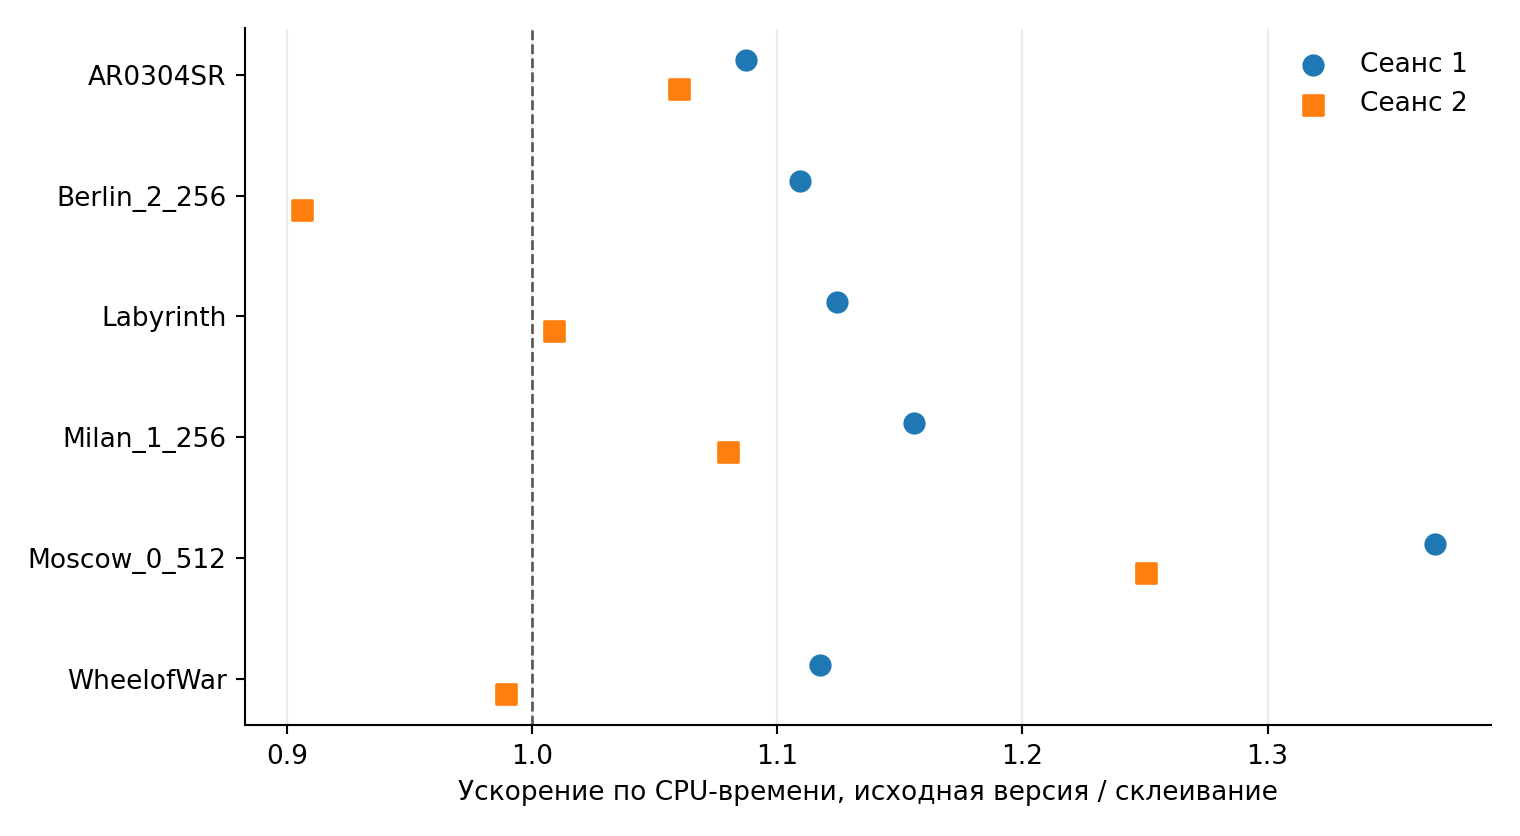
\includegraphics[width=0.77\linewidth]{sessions.png}
\end{center}

Код также поддерживает \href{https://man7.org/linux/man-pages/man2/sched_setaffinity.2.html}{\code{sched_setaffinity}} в Linux. Там выбирается разрешённое ядро и проверяется результат закрепления. Linux-прогон здесь не выполнялся. Полученные проценты относятся к этому Mac и этим наборам задач.

В \href{../results/confirm/manifest.json}{журнале основной серии} сохранены команды, порядок, семена и хеши бинарников. \href{../data_manifest.json}{Манифест данных} и \href{../snapshot_hashes.json}{контрольные суммы исходников} позволяют проверить входные файлы. Сырые CSV сохранены для каждого процесса. Никакие неудобные повторы из основной серии не удалялись.

{\small Команды из корня распакованного проекта:}
\begin{Verbatim}[fontsize=\footnotesize]
bash research/gluing/build.sh
caffeinate -i python3 research/gluing/run_confirm.py
python3 research/gluing/analyze.py
python3 research/gluing/run_holdout.py
python3 research/gluing/profile.py
\end{Verbatim}

В Linux запускать \code{run_confirm.py} без \code{caffeinate}. Компилятор задаётся через \code{CXX}. Для измерений нужны Python 3 и компилятор C++17. Для графика нужен matplotlib.

CLI собирается скриптом \code{research/gluing/build_cli.sh}. Бинарник \code{mesh_astar_glued} принимает авторские аргументы. На примере с обходом стены стоимость осталась 74,4033, число раскрытий уменьшилось с 91\,451 до 69\,586. Разовые времена CLI в оценку ускорения не входят.

\href{../gluing.patch}{Патч}\quad\href{../macro_paths.hpp}{Таблицы цепочек}\quad
\href{../prepare.py}{Изменения генерации потомков}\par
\href{../results/confirmation_summary.json}{Основные результаты}\quad
\href{../results/holdout/summary.json}{Отложенные карты}

\end{document}
